\chapter{Algoritmi s drugim korijenom}

\index{algoritam s drugim korijenom}

\key{Algoritam s drugim korijenom} je algoritam
koji u svojoj vremenskoj složenosti sadrži drugi korijen.
Drugi korijen možemo shvatiti kao ''logaritam za siromašne'':
složenost $O(\sqrt n)$ bolja je od $O(n)$,
ali lošija od $O(\log n)$.
U svakom slučaju, mnogi algoritmi s drugim korijenom brzi su i praktično upotrebljivi.

Kao primjer, razmotrimo zadatak
izgradnje strukture podataka koja podržava
dvije operacije nad nizom:
promjenu elementa na zadanoj poziciji
i računanje sume elemenata na zadanom intervalu.
Taj smo zadatak već riješili pomoću
binarno indeksiranih i segmentnih stabala,
koja obje operacije podržavaju u $O(\log n)$ vremenu.
No sada ćemo zadatak riješiti
na drugi način, pomoću strukture s drugim korijenom
koja nam omogućuje mijenjanje elemenata u $O(1)$ vremenu
i računanje suma u $O(\sqrt n)$ vremenu.

Ideja je podijeliti niz na \emph{blokove}
veličine $\sqrt n$ tako da svaki blok sadrži
sumu elemenata unutar bloka.
Na primjer, niz od 16 elemenata bit će
podijeljen na blokove od 4 elementa ovako:

\begin{center}
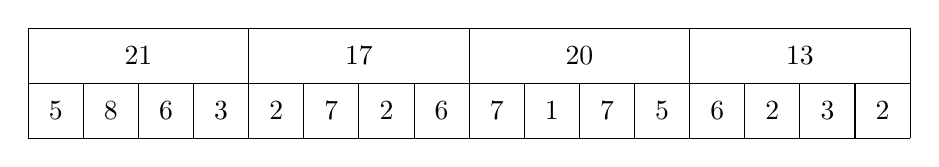
\begin{tikzpicture}[scale=0.7]
\draw (0,0) grid (16,1);

\draw (0,1) rectangle (4,2);
\draw (4,1) rectangle (8,2);
\draw (8,1) rectangle (12,2);
\draw (12,1) rectangle (16,2);

\node at (0.5, 0.5) {5};
\node at (1.5, 0.5) {8};
\node at (2.5, 0.5) {6};
\node at (3.5, 0.5) {3};
\node at (4.5, 0.5) {2};
\node at (5.5, 0.5) {7};
\node at (6.5, 0.5) {2};
\node at (7.5, 0.5) {6};
\node at (8.5, 0.5) {7};
\node at (9.5, 0.5) {1};
\node at (10.5, 0.5) {7};
\node at (11.5, 0.5) {5};
\node at (12.5, 0.5) {6};
\node at (13.5, 0.5) {2};
\node at (14.5, 0.5) {3};
\node at (15.5, 0.5) {2};

\node at (2, 1.5) {21};
\node at (6, 1.5) {17};
\node at (10, 1.5) {20};
\node at (14, 1.5) {13};

\end{tikzpicture}
\end{center}

U ovoj je strukturi
lako mijenjati elemente niza,
jer je nakon svake promjene
potrebno ažurirati samo
sumu jednog bloka,
što se može učiniti u $O(1)$ vremenu.
Na primjer, sljedeća slika prikazuje
kako se mijenjaju vrijednost elementa i
suma pripadajućeg bloka:

\begin{center}
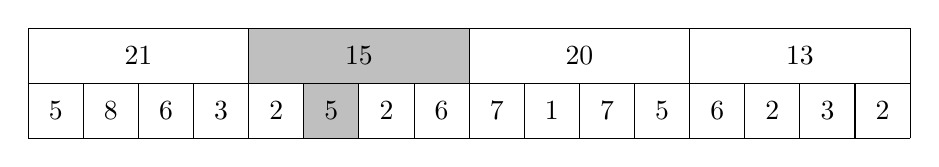
\begin{tikzpicture}[scale=0.7]
\fill[color=lightgray] (5,0) rectangle (6,1);
\draw (0,0) grid (16,1);

\fill[color=lightgray] (4,1) rectangle (8,2);
\draw (0,1) rectangle (4,2);
\draw (4,1) rectangle (8,2);
\draw (8,1) rectangle (12,2);
\draw (12,1) rectangle (16,2);

\node at (0.5, 0.5) {5};
\node at (1.5, 0.5) {8};
\node at (2.5, 0.5) {6};
\node at (3.5, 0.5) {3};
\node at (4.5, 0.5) {2};
\node at (5.5, 0.5) {5};
\node at (6.5, 0.5) {2};
\node at (7.5, 0.5) {6};
\node at (8.5, 0.5) {7};
\node at (9.5, 0.5) {1};
\node at (10.5, 0.5) {7};
\node at (11.5, 0.5) {5};
\node at (12.5, 0.5) {6};
\node at (13.5, 0.5) {2};
\node at (14.5, 0.5) {3};
\node at (15.5, 0.5) {2};

\node at (2, 1.5) {21};
\node at (6, 1.5) {15};
\node at (10, 1.5) {20};
\node at (14, 1.5) {13};

\end{tikzpicture}
\end{center}

Zatim, kako bismo izračunali sumu elemenata na intervalu,
interval dijelimo na tri dijela tako da se
suma sastoji od vrijednosti pojedinačnih elemenata
i suma blokova između njih:

\begin{center}
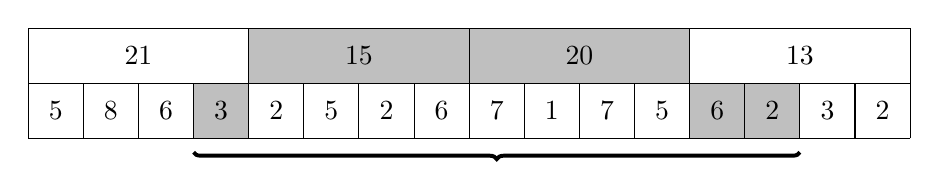
\begin{tikzpicture}[scale=0.7]
\fill[color=lightgray] (3,0) rectangle (4,1);
\fill[color=lightgray] (12,0) rectangle (13,1);
\fill[color=lightgray] (13,0) rectangle (14,1);
\draw (0,0) grid (16,1);

\fill[color=lightgray] (4,1) rectangle (8,2);
\fill[color=lightgray] (8,1) rectangle (12,2);
\draw (0,1) rectangle (4,2);
\draw (4,1) rectangle (8,2);
\draw (8,1) rectangle (12,2);
\draw (12,1) rectangle (16,2);

\node at (0.5, 0.5) {5};
\node at (1.5, 0.5) {8};
\node at (2.5, 0.5) {6};
\node at (3.5, 0.5) {3};
\node at (4.5, 0.5) {2};
\node at (5.5, 0.5) {5};
\node at (6.5, 0.5) {2};
\node at (7.5, 0.5) {6};
\node at (8.5, 0.5) {7};
\node at (9.5, 0.5) {1};
\node at (10.5, 0.5) {7};
\node at (11.5, 0.5) {5};
\node at (12.5, 0.5) {6};
\node at (13.5, 0.5) {2};
\node at (14.5, 0.5) {3};
\node at (15.5, 0.5) {2};

\node at (2, 1.5) {21};
\node at (6, 1.5) {15};
\node at (10, 1.5) {20};
\node at (14, 1.5) {13};

\draw [decoration={brace}, decorate, line width=0.5mm] (14,-0.25) -- (3,-0.25);

\end{tikzpicture}
\end{center}

Budući da je broj pojedinačnih elemenata $O(\sqrt n)$,
a i broj blokova je $O(\sqrt n)$,
upit za sumu traje $O(\sqrt n)$ vremena.
Svrha veličine bloka $\sqrt n$ jest
da ona \emph{uravnotežuje} dvije stvari:
niz je podijeljen na $\sqrt n$ blokova,
od kojih svaki sadrži $\sqrt n$ elemenata.

U praksi nije nužno koristiti
točnu vrijednost $\sqrt n$ kao parametar,
nego možemo koristiti parametre $k$ i $n/k$ gdje je $k$
različit od $\sqrt n$.
Optimalan parametar ovisi o zadatku i ulazu.
Na primjer, ako algoritam često prolazi
kroz blokove, a rijetko pregledava
pojedinačne elemente unutar blokova,
može biti dobra ideja podijeliti niz na
$k < \sqrt n$ blokova, od kojih svaki sadrži $n/k > \sqrt n$
elemenata.

\section{Kombiniranje algoritama}

U ovom odjeljku razmatramo dva algoritma s drugim korijenom
koji se temelje na spajanju dvaju algoritama u jedan algoritam.
U oba slučaja mogli bismo upotrijebiti bilo koji od tih algoritama
bez onog drugog
i riješiti zadatak u $O(n^2)$ vremenu.
No kombiniranjem algoritama vrijeme
izvođenja iznosi samo $O(n \sqrt n)$.

\subsubsection{Obrada po slučajevima}

Pretpostavimo da nam je zadana dvodimenzionalna
mreža koja sadrži $n$ ćelija.
Svakoj je ćeliji pridijeljeno slovo,
a naš je zadatak pronaći dvije ćelije
s istim slovom čija je udaljenost minimalna,
pri čemu je udaljenost između ćelija
$(x_1,y_1)$ i $(x_2,y_2)$ jednaka $|x_1-x_2|+|y_1-y_2|$.
Na primjer, razmotrimo sljedeću mrežu:

\begin{center}
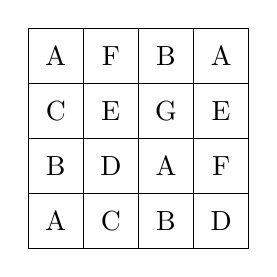
\begin{tikzpicture}[scale=0.7]
\node at (0.5,0.5) {A};
\node at (0.5,1.5) {B};
\node at (0.5,2.5) {C};
\node at (0.5,3.5) {A};
\node at (1.5,0.5) {C};
\node at (1.5,1.5) {D};
\node at (1.5,2.5) {E};
\node at (1.5,3.5) {F};
\node at (2.5,0.5) {B};
\node at (2.5,1.5) {A};
\node at (2.5,2.5) {G};
\node at (2.5,3.5) {B};
\node at (3.5,0.5) {D};
\node at (3.5,1.5) {F};
\node at (3.5,2.5) {E};
\node at (3.5,3.5) {A};
\draw (0,0) grid (4,4);
\end{tikzpicture}
\end{center}
U ovom je slučaju minimalna udaljenost 2, i to između dvaju slova 'E'.

Zadatak možemo riješiti tako da svako slovo promatramo zasebno.
Uz taj pristup, novi je zadatak izračunati
minimalnu udaljenost
između dviju ćelija s \emph{fiksnim} slovom $c$.
Usredotočimo se na dva algoritma za to:

\emph{Algoritam 1:} Prođemo kroz sve parove ćelija sa slovom $c$
i izračunamo minimalnu udaljenost između takvih ćelija.
To će trajati $O(k^2)$ vremena, gdje je $k$ broj ćelija sa slovom $c$.

\emph{Algoritam 2:} Provedemo pretraživanje u širinu koje istovremeno
kreće iz svake ćelije sa slovom $c$. Minimalna udaljenost između
dviju ćelija sa slovom $c$ bit će izračunata u $O(n)$ vremenu.

Jedan način rješavanja zadatka jest odabrati jedan od
tih algoritama i koristiti ga za sva slova.
Ako koristimo Algoritam 1, vrijeme izvođenja je $O(n^2)$,
jer sve ćelije mogu sadržavati isto slovo,
a u tom je slučaju $k=n$.
Također, ako koristimo Algoritam 2, vrijeme izvođenja je $O(n^2)$,
jer sve ćelije mogu imati različita slova,
a u tom je slučaju potrebno $n$ pretraživanja.

Međutim, ta dva algoritma možemo \emph{kombinirati} i
koristiti različite algoritme za različita slova,
ovisno o tome koliko se puta svako slovo pojavljuje u mreži.
Pretpostavimo da se slovo $c$ pojavljuje $k$ puta.
Ako je $k \le \sqrt n$, koristimo Algoritam 1, a ako je $k > \sqrt n$,
koristimo Algoritam 2.
Ispada da je ovakvim postupkom ukupno vrijeme izvođenja
algoritma samo $O(n \sqrt n)$.

Najprije pretpostavimo da za slovo $c$ koristimo Algoritam 1.
Budući da se $c$ u mreži pojavljuje najviše $\sqrt n$ puta,
svaku ćeliju sa slovom $c$ uspoređujemo $O(\sqrt n)$ puta
s drugim ćelijama.
Dakle, vrijeme utrošeno na obradu svih takvih ćelija je $O(n \sqrt n)$.
Zatim pretpostavimo da za slovo $c$ koristimo Algoritam 2.
Takvih slova ima najviše $\sqrt n$,
pa i obrada tih slova traje $O(n \sqrt n)$ vremena.

\subsubsection{Obrada u serijama}

Naš sljedeći zadatak također se bavi
dvodimenzionalnom mrežom koja sadrži $n$ ćelija.
Na početku je svaka ćelija osim jedne bijela.
Izvodimo $n-1$ operaciju, od kojih svaka najprije
izračuna minimalnu udaljenost od zadane bijele ćelije
do crne ćelije, a zatim tu bijelu ćeliju oboji u crno.

Na primjer, razmotrimo sljedeću operaciju:

\begin{center}
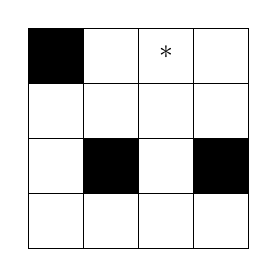
\begin{tikzpicture}[scale=0.7]
\fill[color=black] (1,1) rectangle (2,2);
\fill[color=black] (3,1) rectangle (4,2);
\fill[color=black] (0,3) rectangle (1,4);
\node at (2.5,3.5) {*};
\draw (0,0) grid (4,4);
\end{tikzpicture}
\end{center}

Najprije izračunamo minimalnu udaljenost
od bijele ćelije označene sa * do crne ćelije.
Minimalna udaljenost je 2, jer se možemo pomaknuti
dva koraka ulijevo do crne ćelije.
Zatim bijelu ćeliju obojimo u crno:

\begin{center}
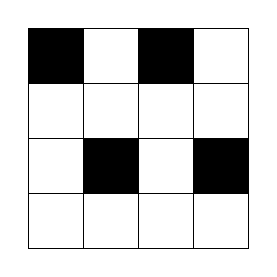
\begin{tikzpicture}[scale=0.7]
\fill[color=black] (1,1) rectangle (2,2);
\fill[color=black] (3,1) rectangle (4,2);
\fill[color=black] (0,3) rectangle (1,4);
\fill[color=black] (2,3) rectangle (3,4);
\draw (0,0) grid (4,4);
\end{tikzpicture}
\end{center}

Razmotrimo sljedeća dva algoritma:

\emph{Algoritam 1:} Pomoću pretraživanja u širinu
izračunamo
za svaku bijelu ćeliju udaljenost do najbliže crne ćelije.
To traje $O(n)$ vremena, a nakon pretraživanja
minimalnu udaljenost od bilo koje bijele ćelije
do crne ćelije možemo pronaći u $O(1)$ vremenu.

\emph{Algoritam 2:} Održavamo listu ćelija koje su
obojene u crno, prolazimo kroz tu listu pri svakoj operaciji
i zatim dodajemo novu ćeliju u listu.
Operacija traje $O(k)$ vremena, gdje je $k$ duljina liste.

Gornje algoritme kombiniramo tako da
operacije podijelimo u
$O(\sqrt n)$ \emph{serija}, od kojih se svaka sastoji
od $O(\sqrt n)$ operacija.
Na početku svake serije
izvedemo Algoritam 1.
Zatim koristimo Algoritam 2 za obradu operacija
u toj seriji.
Listu Algoritma 2 praznimo između
serija.
Pri svakoj operaciji
minimalna udaljenost do crne ćelije
jest ili udaljenost izračunata Algoritmom 1
ili udaljenost izračunata Algoritmom 2.

Dobiveni algoritam radi u
$O(n \sqrt n)$ vremenu.
Prvo, Algoritam 1 izvodi se $O(\sqrt n)$ puta,
a svako pretraživanje radi u $O(n)$ vremenu.
Drugo, kad u seriji koristimo Algoritam 2,
lista sadrži $O(\sqrt n)$ ćelija
(jer listu praznimo između serija)
i svaka operacija traje $O(\sqrt n)$ vremena.

\section{Rastavi cijelih brojeva}

Neki se algoritmi s drugim korijenom temelje na
sljedećem zapažanju:
ako je pozitivan cijeli broj $n$ prikazan kao
suma pozitivnih cijelih brojeva,
takva suma uvijek sadrži najviše
$O(\sqrt n)$ \emph{različitih} brojeva.
Razlog je taj što bismo, da bismo konstruirali
sumu koja sadrži najveći broj različitih
brojeva, trebali birati \emph{male} brojeve.
Ako odaberemo brojeve $1,2,\ldots,k$,
dobivena suma iznosi
\[\frac{k(k+1)}{2}.\]
Dakle, najveća količina različitih brojeva je $k = O(\sqrt n)$.
U nastavku ćemo razmotriti dva zadatka koja se pomoću tog
zapažanja mogu riješiti efikasno.

\subsubsection{Problem naprtnjače}

Pretpostavimo da nam je zadana lista cjelobrojnih težina
čija je suma $n$.
Naš je zadatak pronaći sve sume koje se mogu tvoriti
pomoću nekog podskupa težina. Na primjer, ako su težine
$\{1,3,3\}$, moguće su sume sljedeće:

\begin{itemize}[noitemsep]
\item $0$ (prazan skup)
\item $1$
\item $3$
\item $1+3=4$
\item $3+3=6$
\item $1+3+3=7$
\end{itemize}

Koristeći standardni pristup naprtnjači (vidi poglavlje 7.4),
zadatak se može riješiti ovako:
definiramo funkciju $\texttt{possible}(x,k)$ čija je vrijednost 1
ako se suma $x$ može tvoriti pomoću prvih $k$ težina,
a 0 inače.
Budući da je suma težina $n$,
postoji najviše $n$ težina i
sve vrijednosti funkcije mogu se izračunati
u $O(n^2)$ vremenu pomoću dinamičkog programiranja.

Međutim, algoritam možemo učiniti efikasnijim
koristeći činjenicu da postoji najviše $O(\sqrt n)$
\emph{različitih} težina.
Stoga težine možemo obrađivati u grupama
koje se sastoje od jednakih težina.
Svaku grupu možemo obraditi
u $O(n)$ vremenu, što daje algoritam vremenske složenosti $O(n \sqrt n)$.

Ideja je koristiti niz koji bilježi sume težina
koje se mogu tvoriti pomoću dosad obrađenih grupa.
Niz sadrži $n$ elemenata: element $k$ je 1 ako se suma
$k$ može tvoriti, a 0 inače.
Da bismo obradili grupu težina, prolazimo nizom
slijeva nadesno i bilježimo nove sume težina koje
se mogu tvoriti pomoću te grupe i prethodnih grupa.

\subsubsection{Konstrukcija znakovnog niza}

Zadan je znakovni niz \texttt{s} duljine $n$
i skup znakovnih nizova $D$ čija je ukupna duljina $m$;
razmotrimo zadatak prebrojavanja broja načina na koje se
\texttt{s} može tvoriti kao nadovezivanje znakovnih nizova iz $D$.
Na primjer,
ako je $\texttt{s}=\texttt{ABAB}$ i
$D=\{\texttt{A},\texttt{B},\texttt{AB}\}$,
postoje 4 načina:

\begin{itemize}[noitemsep]
\item $\texttt{A}+\texttt{B}+\texttt{A}+\texttt{B}$
\item $\texttt{AB}+\texttt{A}+\texttt{B}$
\item $\texttt{A}+\texttt{B}+\texttt{AB}$
\item $\texttt{AB}+\texttt{AB}$
\end{itemize}

Zadatak možemo riješiti pomoću dinamičkog programiranja:
neka $\texttt{count}(k)$ označava broj načina na koje se prefiks
$\texttt{s}[0 \ldots k]$ može konstruirati pomoću znakovnih nizova iz $D$.
Sada $\texttt{count}(n-1)$ daje odgovor na zadatak,
a zadatak možemo riješiti u $O(n^2)$ vremenu
pomoću trie strukture.

Međutim, zadatak možemo riješiti efikasnije
koristeći raspršivanje znakovnih nizova i činjenicu da u $D$
postoji najviše $O(\sqrt m)$ različitih duljina znakovnih nizova.
Najprije konstruiramo skup $H$ koji sadrži sve
hash vrijednosti znakovnih nizova iz $D$.
Zatim, pri računanju vrijednosti $\texttt{count}(k)$,
prolazimo kroz sve vrijednosti $p$
takve da u $D$ postoji znakovni niz duljine $p$,
izračunamo hash vrijednost od $\texttt{s}[k-p+1 \ldots k]$
i provjerimo pripada li ona skupu $H$.
Budući da postoji najviše $O(\sqrt m)$ različitih duljina znakovnih nizova,
ovo daje algoritam čije je vrijeme izvođenja $O(n \sqrt m)$.

\section{Mo-ov algoritam}

\index{Mo-ov algoritam}

\key{Mo-ov algoritam}\footnote{Prema \cite{cod15}, ovaj je algoritam
nazvan po Mo Taou, kineskom natjecateljskom programeru, no
tehnika se ranije pojavila u literaturi \cite{ken06}.}
može se koristiti u mnogim zadacima
koji zahtijevaju obradu upita nad intervalima u
\emph{statičnom} nizu, tj. vrijednosti niza
ne mijenjaju se između upita.
U svakom upitu zadan nam je interval $[a,b]$,
a trebamo izračunati vrijednost na temelju
elemenata niza između pozicija $a$ i $b$.
Budući da je niz statičan,
upiti se mogu obrađivati bilo kojim redoslijedom,
a Mo-ov algoritam
obrađuje upite u posebnom redoslijedu koji jamči
da algoritam radi efikasno.

Mo-ov algoritam održava \emph{aktivni interval}
niza, a odgovor na upit
koji se odnosi na aktivni interval poznat je u svakom trenutku.
Algoritam obrađuje upite jedan po jedan
i uvijek pomiče krajeve
aktivnog intervala umetanjem i uklanjanjem elemenata.
Vremenska složenost algoritma je
$O(n \sqrt n f(n))$, gdje niz sadrži
$n$ elemenata, ima $n$ upita
i svako umetanje i uklanjanje elementa
traje $O(f(n))$ vremena.

Trik Mo-ovog algoritma je u redoslijedu
kojim se upiti obrađuju:
niz je podijeljen na blokove od $k=O(\sqrt n)$
elemenata, a upit $[a_1,b_1]$
obrađuje se prije upita $[a_2,b_2]$
ako vrijedi ili
\begin{itemize}
\item $\lfloor a_1/k \rfloor < \lfloor a_2/k \rfloor$ ili
\item $\lfloor a_1/k \rfloor = \lfloor a_2/k \rfloor$ i $b_1 < b_2$.
\end{itemize}

Dakle, svi upiti čiji su lijevi krajevi
u određenom bloku obrađuju se jedan za drugim,
sortirani prema svojim desnim krajevima.
Uz taj redoslijed algoritam
izvodi samo $O(n \sqrt n)$ operacija,
jer se lijevi kraj pomiče
$O(n)$ puta po $O(\sqrt n)$ koraka,
a desni se kraj pomiče
$O(\sqrt n)$ puta po $O(n)$ koraka. Dakle, oba se
kraja tijekom algoritma pomaknu ukupno $O(n \sqrt n)$ koraka.

\subsubsection*{Primjer}

Kao primjer, razmotrimo zadatak
u kojem nam je zadan skup upita,
od kojih svaki odgovara nekom intervalu u nizu,
a naš je zadatak za svaki upit izračunati
broj \emph{različitih} elemenata u tom intervalu.

U Mo-ovom algoritmu upiti se uvijek sortiraju
na isti način, no o zadatku ovisi
kako se održava odgovor na upit.
U ovom zadatku možemo održavati niz
\texttt{count} u kojem $\texttt{count}[x]$
označava koliko se puta element $x$
pojavljuje u aktivnom intervalu.

Kada prelazimo s jednog upita na drugi,
aktivni se interval mijenja.
Na primjer, ako je trenutni interval
\begin{center}
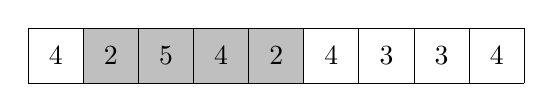
\begin{tikzpicture}[scale=0.7]
\fill[color=lightgray] (1,0) rectangle (5,1);
\draw (0,0) grid (9,1);
\node at (0.5, 0.5) {4};
\node at (1.5, 0.5) {2};
\node at (2.5, 0.5) {5};
\node at (3.5, 0.5) {4};
\node at (4.5, 0.5) {2};
\node at (5.5, 0.5) {4};
\node at (6.5, 0.5) {3};
\node at (7.5, 0.5) {3};
\node at (8.5, 0.5) {4};
\end{tikzpicture}
\end{center}
a sljedeći je interval
\begin{center}
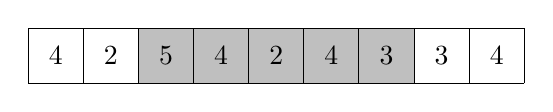
\begin{tikzpicture}[scale=0.7]
\fill[color=lightgray] (2,0) rectangle (7,1);
\draw (0,0) grid (9,1);
\node at (0.5, 0.5) {4};
\node at (1.5, 0.5) {2};
\node at (2.5, 0.5) {5};
\node at (3.5, 0.5) {4};
\node at (4.5, 0.5) {2};
\node at (5.5, 0.5) {4};
\node at (6.5, 0.5) {3};
\node at (7.5, 0.5) {3};
\node at (8.5, 0.5) {4};
\end{tikzpicture}
\end{center}
bit će potrebna tri koraka:
lijevi se kraj pomiče jedan korak udesno,
a desni se kraj pomiče dva koraka udesno.

Nakon svakog koraka niz \texttt{count}
treba ažurirati.
Nakon dodavanja elementa $x$
povećamo vrijednost
$\texttt{count}[x]$ za 1,
i ako je nakon toga $\texttt{count}[x]=1$,
također povećamo odgovor na upit za 1.
Slično, nakon uklanjanja elementa $x$
smanjimo vrijednost
$\texttt{count}[x]$ za 1,
i ako je nakon toga $\texttt{count}[x]=0$,
također smanjimo odgovor na upit za 1.

U ovom zadatku vrijeme potrebno za izvođenje
svakog koraka je $O(1)$, pa je ukupna vremenska složenost
algoritma $O(n \sqrt n)$.